\documentclass[12pt,a4paper]{ctexart}

\usepackage{geometry}
\usepackage{graphicx}
\usepackage{array}
\usepackage{booktabs}
\usepackage{xeCJK}
\usepackage{tikz}
\usepackage{titlesec}
\usepackage{amsmath}
\usepackage{amssymb}

% 页面设置
\geometry{
    top=2.5cm,
    bottom=2.5cm,
    left=2.8cm,
    right=2.8cm
}

% 定义 section* 格式
\titleformat{\section}
  {\zihao{-3}\heiti\bfseries}
  {}
  {0em}
  {}
\titlespacing*{\section}{0pt}{0.5cm}{0.3cm}  % 左缩进、上间距、下间距


% 取消页码（封面）
\pagestyle{empty}

% 定义等长下划线命令（固定宽度 6.5cm，左对齐）
\newcommand{\infofill}[1]{{\zihao{4}\songti\underline{\makebox[6.5cm][c]{#1}}}}

% 定义内容区块命令
\newcommand{\reportsection}[2]{%
    \noindent{\zihao{-3}\heiti\bfseries #1（#2分）}
    \vspace{0.3cm}
    
    \noindent\rule{\textwidth}{0.4pt}
    \vspace{6cm}
}

% 设置中文字体
\setCJKmainfont{SimSun}  % 宋体，可根据系统改为 Noto Serif CJK SC 等

\begin{document}
% ==================== 封面页 ====================
\begin{titlepage}
    \centering
    \vspace*{1.5cm}
    % 校徽占位（正方形示例图）
    
\includegraphics[width=5cm,height=5cm]{images/image-2026-09-07-14-57-04.png}
    
    \vspace{1.8cm}
    
    % 中山大学
    {\zihao{1}\heiti\bfseries 中山大学}
    
    \vspace{0.9cm}
    
    % 微电子科学与技术学院
    {\zihao{2}\heiti 微电子科学与技术学院}
    
    \vspace{0.9cm}
    
    % 课程名称
    {\zihao{2}\heiti 《集成电路元器件特性表征实验》}
    
    \vspace{0.9cm}
    
    % 实验报告
    {\zihao{1}\heiti\bfseries 实验报告}
    
    \vspace{3cm}
    
    % 信息表格
    

    % 信息表格（无任何框线，无横线，无竖线）
    \begin{tabular}{@{}>{\zihao{4}\heiti}r @{\hspace{1.2em}} l@{}}
        实验主题      & \infofill{PN 结的电容-电压特性测试实验}        \\[0.8cm]
        姓\quad\quad 名 & \infofill{徐睿琳}   \\[0.8cm]
        学\quad\quad 号 & \infofill{23342107} \\[0.8cm]
        实验日期      & \infofill{\today}   \\[0.8cm]
    \end{tabular}
    
    \vfill
\end{titlepage}

% ==================== 内容页 ====================
\newpage
\pagestyle{plain}
\setcounter{page}{2}

\section*{实验目的（5分）}

\begin{enumerate}
    \item 掌握 PN 结耗尽层电容的物理起源，理解反向偏压下微分电容 $C$ 与偏压 $V$ 的理论关系及 $1/C^{2}$--$V$ 线性化的依据。
    \item 掌握 TH1992B 源表与 TH2840B LCR 表联用的偏置扫描测试方法，正确获取 HER303 二极管的 $C$--$V$ 特性数据。
    \item 掌握由 $1/C^{2}$--$V$ 曲线外推截距求内建电势 $V_{bi}$，并由
    $N_B=\dfrac{2}{A^{2}q\varepsilon_{s}}\left[\dfrac{\mathrm{d}(1/C^{2})}{\mathrm{d}V}\right]^{-1}$
    求轻掺杂侧掺杂浓度及其纵向分布的数据处理方法，验证单边突变结近似的适用性。
\end{enumerate}

\section*{实验原理（10分）}

\subsection*{1. 耗尽层电容的物理起源}
PN 结接触后因载流子浓度梯度发生扩散，留下不可动电离杂质，形成由 N 区指向 P 区的内建电场与内建电势 $V_{bi}$，电场所在区域即耗尽区（势垒区）。反向偏压 $V$ 几乎全部降落于耗尽区，故耗尽区总电势差为 $V_{bi}-V$，耗尽区宽度随反向偏压增大而展宽，呈现随电压可调的电容效应。

\subsection*{2. 耗尽近似与微分电容}
一维耗尽区内电荷分布与电场满足泊松方程
\begin{equation}
-\frac{\mathrm{d}^{2}V}{\mathrm{d}x^{2}}=\frac{\mathrm{d}E}{\mathrm{d}x}=\frac{\rho(x)}{\varepsilon},\qquad
\rho(x)=q\left[p(x)-n(x)+N_D(x)-N_A(x)\right].
\end{equation}
在耗尽近似下（$\rho=qN_D$ 或 $-qN_A$，$x>L$ 处 $E=0$），积分得耗尽区宽度
\begin{equation}
L=\left[\left(V_{bi}-V\right)\frac{2\varepsilon\left(N_A+N_D\right)}{qN_AN_D}\right]^{1/2}.
\end{equation}
耗尽层微分电容定义为 $C=\left|\mathrm{d}Q/\mathrm{d}V\right|$，由 $C=\varepsilon A/L$ 得
\begin{equation}
C=A\left[\frac{q\varepsilon N_AN_D}{2\left(N_A+N_D\right)\left(V_{bi}-V\right)}\right]^{1/2}.
\end{equation}

\subsection*{3. 单边突变结的 $1/C^{2}$--$V$ 线性化}
HER303 为单边突变结（$N_A\gg N_D$ 或反之），记轻掺杂侧浓度 $N_B$，则
\begin{equation}
C=A\left[\frac{q\varepsilon N_B}{2\left(V_{bi}-V\right)}\right]^{1/2}
\;\Longrightarrow\;
\frac{1}{C^{2}}=\frac{2\left(V_{bi}-V\right)}{A^{2}q\varepsilon N_B}.
\end{equation}
故 $1/C^{2}$ 与 $V$ 呈线性关系：其斜率 $k=-2/(A^{2}q\varepsilon N_B)$ 给出轻掺杂侧掺杂浓度
\begin{equation}
N_B=\frac{2}{A^{2}q\varepsilon}\left[\frac{\mathrm{d}\left(1/C^{2}\right)}{\mathrm{d}V}\right]^{-1}
=-\frac{C^{3}}{A^{2}q\varepsilon}\frac{\mathrm{d}V}{\mathrm{d}C},
\end{equation}
其电压轴截距（$1/C^{2}=0$ 处）即为内建电势 $V_{bi}$。

\subsection*{4. 测试频率的选择}
C--V 测试采用高频小信号：此时少子产生--复合过程来不及跟随交流信号，器件电容仅由耗尽层电离杂质电荷贡献，与式 (4) 相符；低频下少子的充放电将引入额外扩散电容，使 $1/C^{2}$--$V$ 偏离线性并导致 $V_{bi}$、$N_B$ 提取失真。

本实验数据处理统一取 $\varepsilon=10\varepsilon_0$、$A=10\ \mathrm{mm^{2}}$、$q=1.602\times10^{-19}\ \mathrm{C}$。


\section*{实验设备和步骤（5分）}

\subsection*{1. 实验设备}
\begin{itemize}
    \item \textbf{待测样品}：HER303 快恢复二极管（单边突变结，PN 结型）；
    \item \textbf{偏置源}：同惠 TH1992B 源表（CH1），提供扫描直流偏压 $V$；
    \item \textbf{电容测量}：同惠 TH2840B LCR 数字电桥，四端法测结电容 $C$；
    \item \textbf{测试平台}：同惠 TH300E（含屏蔽测试夹具），构成源表--LCR 表--夹具的联合测试回路；
    \item \textbf{上位机}：配套测试软件，完成参数设置、偏置扫描与数据采集。
\end{itemize}

\subsection*{2. 实验步骤}
\begin{enumerate}
    \item \textbf{开机预热}：将 TH300E 电源开关置于 ON，使面板各单元通电预热。
    \item \textbf{接线}：按四端法将测试夹具与 TH2840B LCR 表的测试端连接；TH1992B 源表 CH1 的正、负极分别与夹具正、负极对应连接；将 HER303 样品插入夹具，注意插槽极性与引脚对应，避免反接。
    \item \textbf{参数设置}：开启测试软件，设定偏置扫描范围（本实验 $V=-5\sim+3\ \mathrm{V}$）、步进间隔、交流小信号频率（高频）与信号幅度（小信号，满足线性近似）。
    \item \textbf{扫描测试}：按下开始按钮，由源表逐点施加偏压、LCR 表同步读取电容；加偏置期间禁止用手触摸电极，防止漏电与触电。
    \item \textbf{数据采集}：测试完毕导出 $C$--$V$ 原始数据，作后续 $1/C^{2}$--$V$ 线性化与 $N_B(V)$ 计算。
\end{enumerate}

\section*{实验数据分析（50分）}

\subsection*{1. 原始数据与有效区间判别}
全量程共 100 个数据点，$V=-5\sim+3\ \mathrm{V}$。表~\ref{tab:raw} 给出抽样原始数据，图~\ref{fig:cv} 为 $C$--$V$ 全曲线。按物理规律可将扫描范围划分为四个区间：

\begin{table}[htbp]
\centering\small
\caption{HER303 $C$--$V$ 原始数据抽样}
\label{tab:raw}
\begin{tabular}{@{}cccc|cccc@{}}
\toprule
$V/\mathrm{V}$ & $C/\mathrm{nF}$ & $1/C^{2}/(10^{20}\mathrm{F^{-2}})$ & 区间 &
$V/\mathrm{V}$ & $C/\mathrm{nF}$ & $1/C^{2}/(10^{20}\mathrm{F^{-2}})$ & 区间\\
\midrule
$-5.000$ & 0.08602 & 1.3514 & 异常 & $-1.121$ & 0.07629 & 1.7181 & 有效\\
$-4.677$ & 0.05862 & 2.9106 & 异常 & $-0.475$ & 0.09331 & 1.1484 & 有效\\
$-4.354$ & 0.05001 & 3.9980 & 本底 & $+0.172$ & 0.15795 & 0.4009 & 有效\\
$-3.707$ & 0.05260 & 3.6143 & 本底 & $+0.495$ & 1.20621 & 0.00687 & 导通\\
$-3.061$ & 0.05630 & 3.1546 & 有效 & $+1.141$ & 1.22550 & 0.00666 & 导通\\
$-2.414$ & 0.06076 & 2.7086 & 有效 & $+1.788$ & 1.19988 & 0.00695 & 导通\\
$-1.768$ & 0.06689 & 2.2352 & 有效 & $+3.000$ & 1.21043 & 0.00683 & 导通\\
\bottomrule
\end{tabular}
\end{table}

\begin{figure}[htbp]
\centering
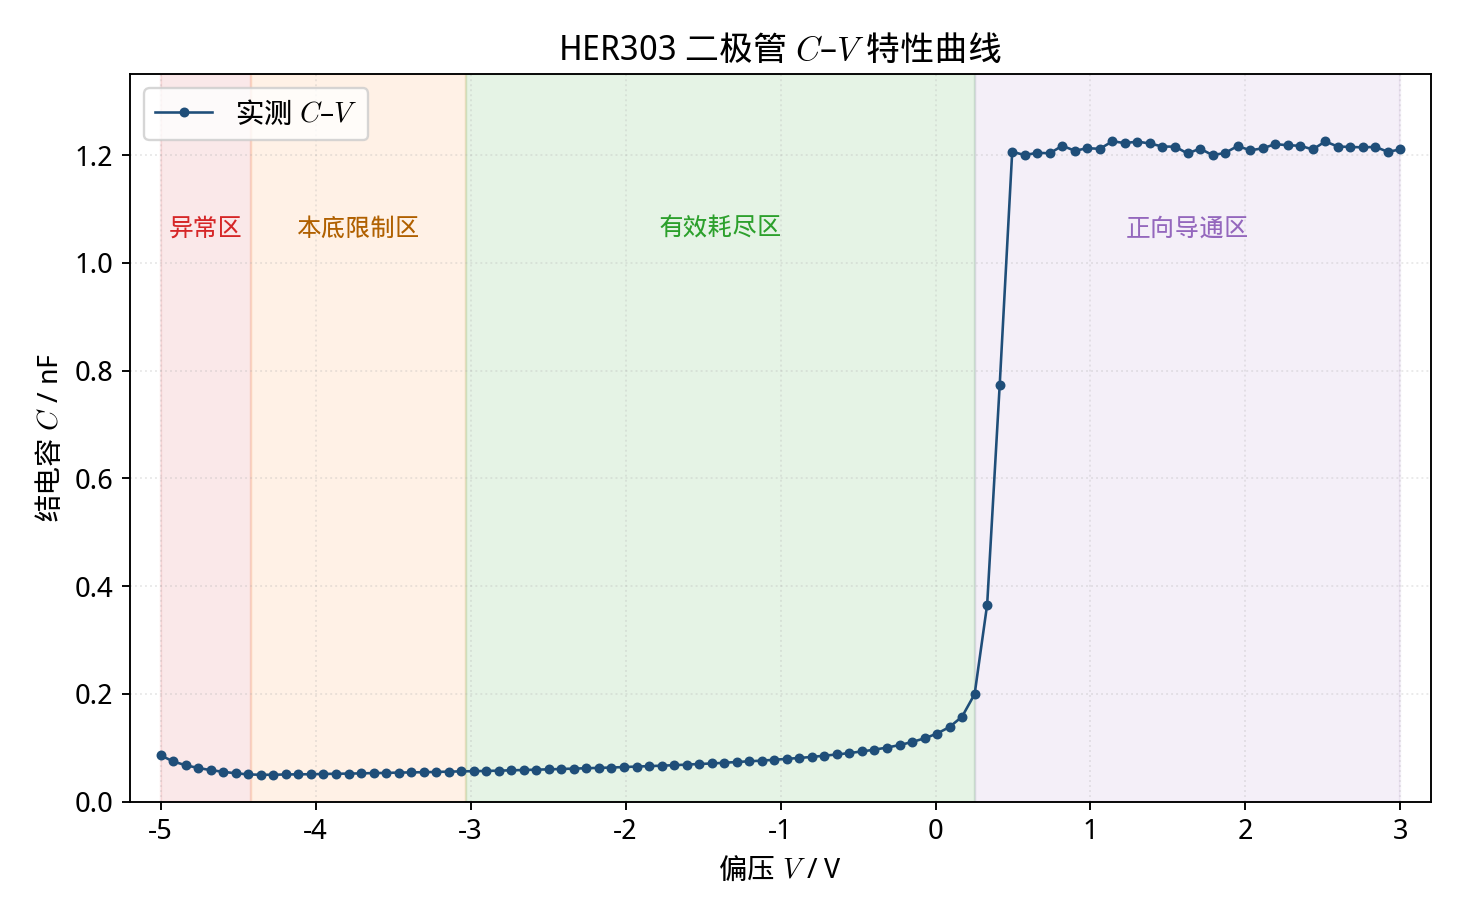
\includegraphics[width=0.82\textwidth]{images/image-fig1_CV.png.png}
\caption{HER303 $C$--$V$ 特性曲线及区间划分}
\label{fig:cv}
\end{figure}

\begin{itemize}
    \item \textbf{异常区（$-5\sim-4.42\ \mathrm{V}$）}：$C$ 随反向偏压减小反而由 0.086 nF 降至 0.050 nF，与耗尽层理论相悖，判定为扫描起始段源表--LCR 表同步未稳定所致，予以剔除；
    \item \textbf{本底限制区（$-4.42\sim-3.03\ \mathrm{V}$）}：$C$ 仅由 0.0500 nF 缓升至 0.0548 nF（变化 $<10\%$），已逼近 LCR 表低电容分辨极限，信噪比不足，不参与拟合；
    \item \textbf{正向导通区（$V>0.33\ \mathrm{V}$）}：$C$ 由 0.20 nF 突增至 0.77 nF 并饱和于 $1.213\pm0.007$ nF，系正向注入引入扩散电容、器件脱离反偏耗尽工作状态，该段数据无效。
\end{itemize}

据此确定\textbf{有效分析区间为 $V\in[-3.03,\,0.25]\ \mathrm{V}$}，共 40 点。

\subsection*{2. $1/C^{2}$--$V$ 线性化与内建电势}
对有效区间内数据作最小二乘线性拟合：
\begin{equation}
\frac{1}{C^{2}}=kV+b,\qquad
k=-8.295\times10^{19}\ \mathrm{F^{-2}{\cdot}V^{-1}},\quad
b=7.280\times10^{19}\ \mathrm{F^{-2}},
\end{equation}
拟合优度 $R^{2}=0.9943$，表明该区间内单边突变结近似成立良好（图~\ref{fig:inv}）。由 $1/C^{2}=0$ 外推得电压轴截距
\begin{equation}
V_{bi}=-\frac{b}{k}=0.878\ \mathrm{V},
\end{equation}
与 Si 突变结内建电势的典型量级（$0.6\sim0.9\ \mathrm{V}$）相符。

\begin{figure}[htbp]
\centering
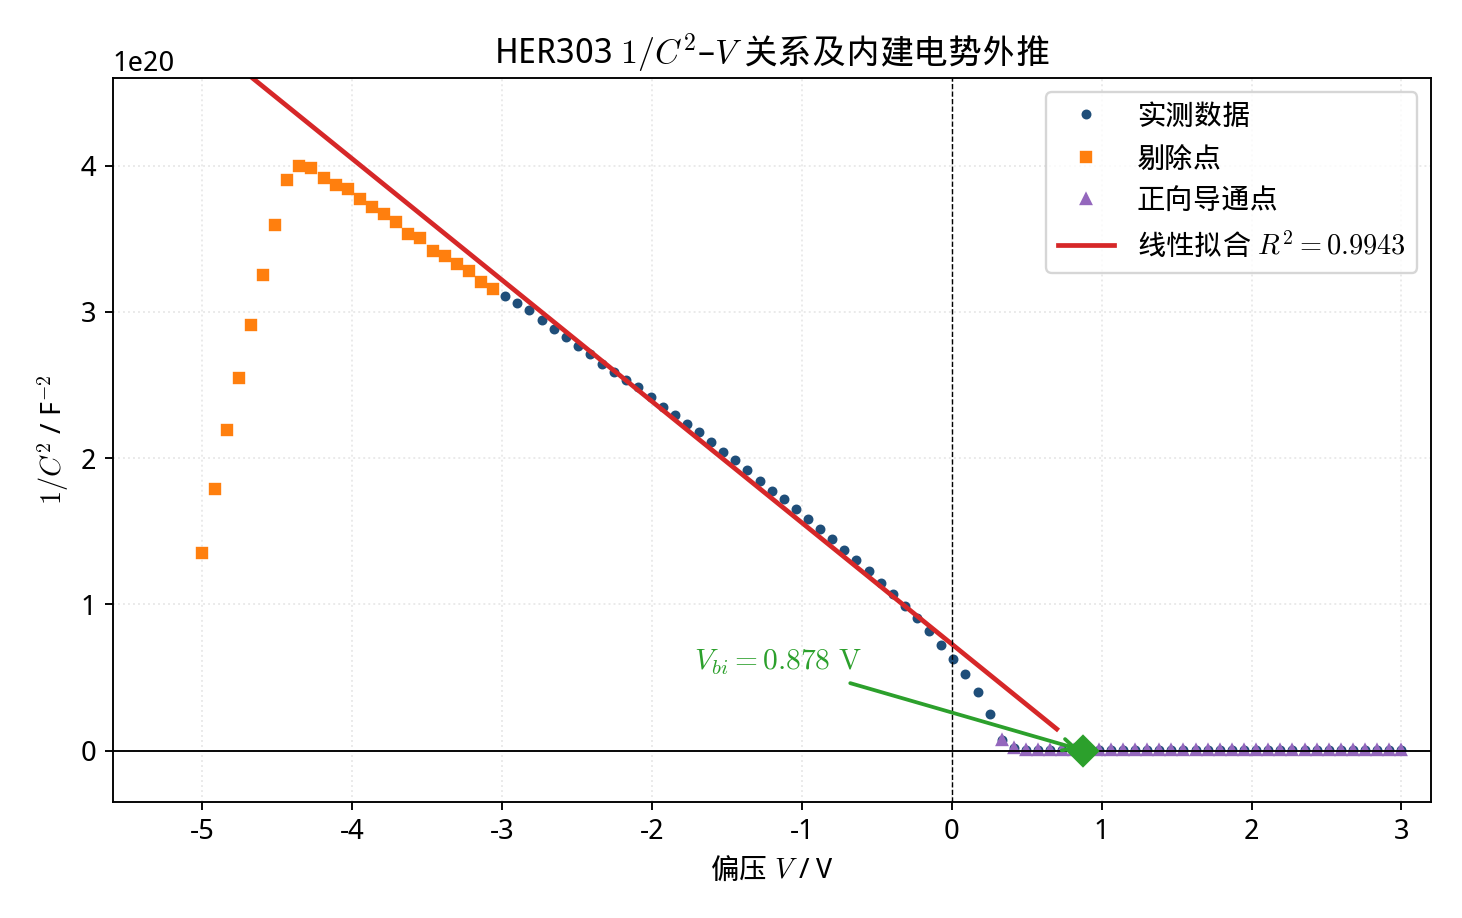
\includegraphics[width=0.82\textwidth]{images/image-2026-09-27-21-30-35.png}
\caption{$1/C^{2}$--$V$ 关系、线性拟合与 $V_{bi}$ 外推}
\label{fig:inv}
\end{figure}

\subsection*{3. 轻掺杂侧掺杂浓度}
取 $\varepsilon=10\varepsilon_0=8.854\times10^{-11}\ \mathrm{F/m}$、$A=10\ \mathrm{mm^{2}}=1.0\times10^{-5}\ \mathrm{m^{2}}$、$q=1.602\times10^{-19}\ \mathrm{C}$，则
\begin{equation}
\frac{2}{A^{2}q\varepsilon}=1.410\times10^{39}\ (\mathrm{SI}),
\qquad
N_B=\frac{2}{A^{2}q\varepsilon}\left(-\frac{1}{k}\right)
=1.700\times10^{19}\ \mathrm{m^{-3}}=1.70\times10^{13}\ \mathrm{cm^{-3}}.
\end{equation}
由 $x=\varepsilon A/C$ 得零偏耗尽宽度 $x_0=7.06\ \mu\mathrm{m}$，有效区内 $x$ 覆盖 $5.61\sim15.61\ \mu\mathrm{m}$。

\subsection*{4. 掺杂浓度纵向分布}
对 $1/C^{2}(V)$ 作 Savitzky--Golay 平滑后逐点求微分，按
$N_B(x)=\dfrac{2}{A^{2}q\varepsilon}\left[\mathrm{d}(1/C^{2})/\mathrm{d}V\right]^{-1}$、$x=\varepsilon A/C$ 换算，得掺杂浓度剖面（图~\ref{fig:nbx}）：$N_B$ 自结区侧 $x=5.6\ \mu\mathrm{m}$ 处的 $1.06\times10^{13}\ \mathrm{cm^{-3}}$ 单调升至深处 $x=15.6\ \mu\mathrm{m}$ 处的 $2.26\times10^{13}\ \mathrm{cm^{-3}}$。

\begin{figure}[htbp]
\centering
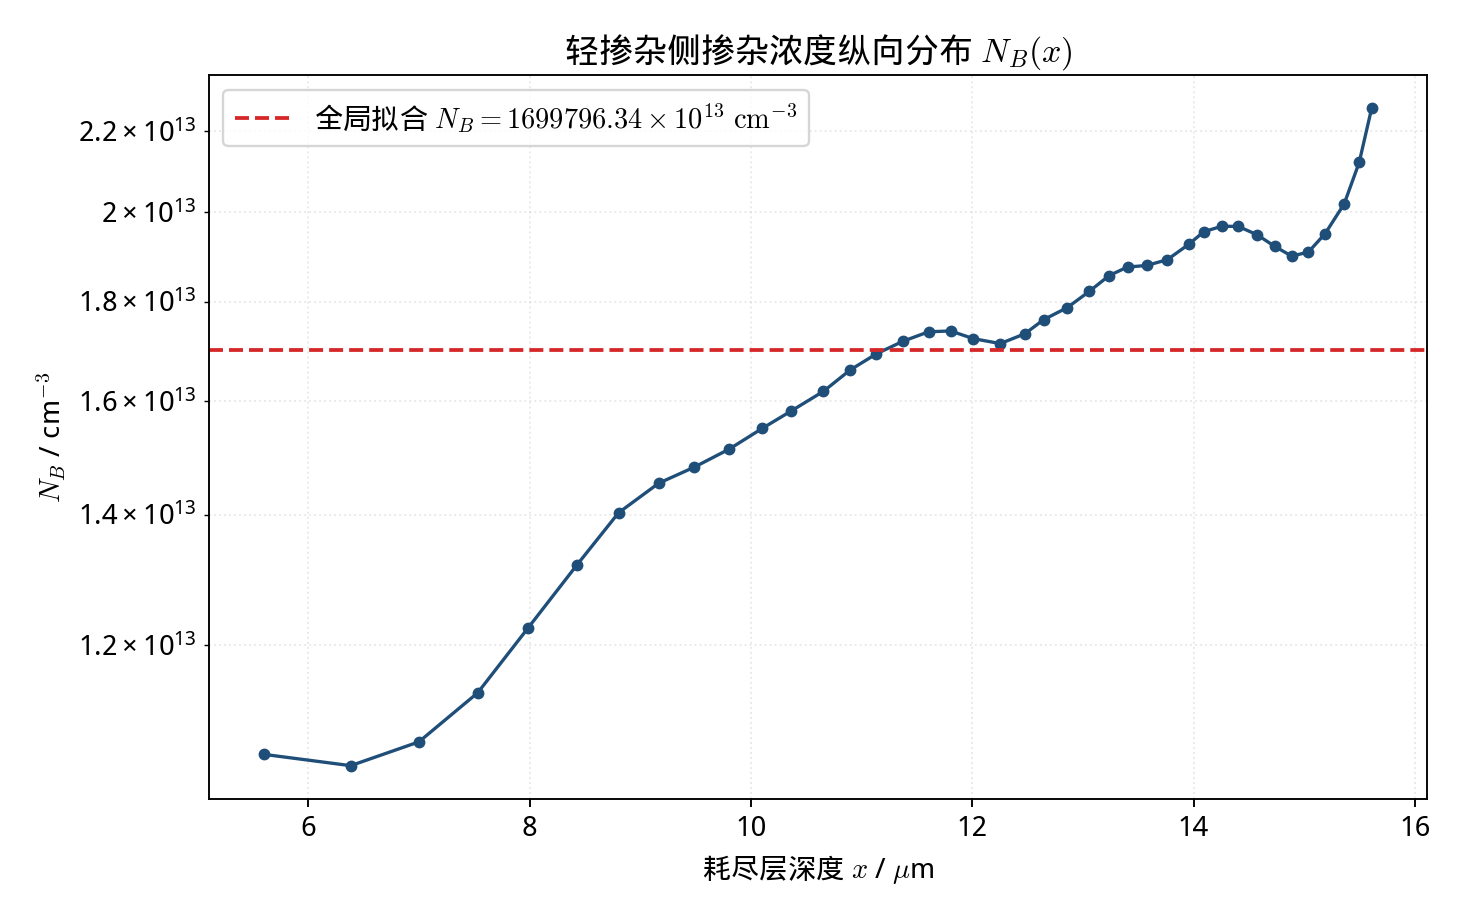
\includegraphics[width=0.82\textwidth]{images/image-2026-09-27-21-30-50.png}
\caption{轻掺杂侧掺杂浓度纵向分布 $N_B(x)$}
\label{fig:nbx}
\end{figure}

\subsection*{5. 拟合窗口稳健性与误差讨论}
改变拟合窗口左端点，考察结果的系统漂移（表~\ref{tab:win}）。

\begin{table}[htbp]
\centering\small
\caption{拟合窗口对提取结果的影响（右端点均取 $0.25\ \mathrm{V}$）}
\label{tab:win}
\begin{tabular}{@{}cccc@{}}
\toprule
窗口左端 $/\mathrm{V}$ & $V_{bi}/\mathrm{V}$ & $N_B/(10^{13}\mathrm{cm^{-3}})$ & $R^{2}$\\
\midrule
$-4.35$ & 1.019 & 1.824 & 0.9944\\
$-3.50$ & 0.937 & 1.756 & 0.9939\\
$-3.03$（采用） & \textbf{0.878} & \textbf{1.700} & 0.9943\\
$-2.50$ & 0.824 & 1.644 & 0.9941\\
$-2.00$ & 0.755 & 1.566 & 0.9940\\
$-1.00$ & 0.623 & 1.376 & 0.9943\\
\bottomrule
\end{tabular}
\end{table}

\begin{itemize}
    \item 各窗口 $R^{2}$ 均 $\geq0.994$，但 $V_{bi}$ 与 $N_B$ 随窗口单调漂移，说明 $1/C^{2}$--$V$ 并非严格直线，而是存在轻微曲率；其物理根源即图~\ref{fig:nbx} 所示的掺杂浓度纵向不均匀，故 $V_{bi}$、$N_B$ 应理解为有效区内的\textbf{平均值}。
    \item 主要误差来源：\textcircled{1} 结面积 $A$ 取统一标称值，$N_B\propto A^{-2}$，$A$ 偏差 10\% 将引入约 20\% 的浓度误差；\textcircled{2} 近本底区（$C\sim50\ \mathrm{pF}$）信噪比低；\textcircled{3} 高频小信号下残余串联电阻与夹具寄生电容未作修正；\textcircled{4} 界面态与可动电荷引起的平带电压漂移会使外推 $V_{bi}$ 偏离真实值。
    \item 结论：HER303 在 $V\in[-3.03,\,0.25]\ \mathrm{V}$ 范围内满足单边突变结耗尽层电容模型，$V_{bi}=0.878\ \mathrm{V}$，轻掺杂侧 $N_B=1.70\times10^{13}\ \mathrm{cm^{-3}}$，且浓度随深度增加呈上升趋势。
\end{itemize}

\section*{实验结论（20分）}

\begin{enumerate}
    \item \textbf{器件类型与模型适用性}：待测样品 HER303 快恢复二极管在反向偏压区 $V\in[-3.03,\,0.25]\ \mathrm{V}$ 内，$1/C^{2}$ 与 $V$ 呈良好线性（$R^{2}=0.9943$），表明其结区在该偏压范围内满足\textbf{单边突变结耗尽层电容模型}，可用耗尽近似与泊松方程描述。
    
    \item \textbf{内建电势}：由 $1/C^{2}$--$V$ 直线的电压轴截距外推得
    \begin{equation}
    V_{bi}=-\frac{b}{k}=\frac{7.280\times10^{19}}{8.295\times10^{19}}=0.878\ \mathrm{V},
    \end{equation}
    与 Si 突变结内建电势的典型量级（$0.6\sim0.9\ \mathrm{V}$）一致，结果合理。
    
    \item \textbf{掺杂浓度}：由直线斜率 $k=-8.295\times10^{19}\ \mathrm{F^{-2}{\cdot}V^{-1}}$ 得轻掺杂一侧浓度
    \begin{equation}
    N_B=\frac{2}{A^{2}q\varepsilon}\left(-\frac{1}{k}\right)=1.70\times10^{13}\ \mathrm{cm^{-3}},
    \end{equation}
    量级与快恢复二极管为获得高耐压而采用的中低掺杂基区设计相符（由 $V_B\propto N_B^{-3/4}$ 可解释其 200 V 级反向耐压）。
    
    \item \textbf{浓度纵向分布}：$N_B(x)$ 自 $x=5.6\ \mu\mathrm{m}$ 处的 $1.06\times10^{13}\ \mathrm{cm^{-3}}$ 单调升至 $x=15.6\ \mu\mathrm{m}$ 处的 $2.26\times10^{13}\ \mathrm{cm^{-3}}$，说明基区掺杂\textbf{并非严格均匀}，而是随深度递增；零偏耗尽宽度 $x_0=\varepsilon A/C_0=7.06\ \mu\mathrm{m}$。
    
    \item \textbf{无效数据段的物理判据}：$V<-4.42\ \mathrm{V}$ 段 $C$ 反常下降，属扫描起始段仪器同步未稳，非本征特性；$-4.42\sim-3.03\ \mathrm{V}$ 段电容钉于约 $50\ \mathrm{pF}$，受 LCR 表低电容分辨本底限制；$V>0.33\ \mathrm{V}$ 后电容骤增并饱和于 $1.213\pm0.007\ \mathrm{nF}$，标志器件进入\textbf{正向导通}，扩散电容主导，耗尽层模型失效。三段均须剔除。
    
    \item \textbf{误差定性结论}：$V_{bi}$ 与 $N_B$ 随拟合窗口单调漂移（$V_{bi}$ 由 0.62 V 至 1.02 V），反映 $1/C^{2}$--$V$ 存在轻微曲率；故所得 $V_{bi}$、$N_B$ 应理解为有效区内的\textbf{等效平均值}。主导误差来自结面积取值（$N_B\propto A^{-2}$）、近本底区低信噪比、串联电阻与夹具寄生未修正。
\end{enumerate}

\section*{实验启示和拓展（10分）}

\subsection*{1. 思考题}
\begin{itemize}
    \item \textbf{PN 结电容的组成}：总电容含两项——\emph{势垒电容}（耗尽层电容 $C_j=\varepsilon A/L$，由耗尽区内电离杂质电荷随偏压变化产生，反偏时占主导）与\emph{扩散电容}（$C_D\propto\tau_F I_F$，由正向注入少子的存储电荷随电压变化产生，正偏时占主导）；另在高频等效中还需计入封装与引线的\emph{寄生电容}。本实验反偏段测得的即 $C_j$。
    \item \textbf{为何选高频}：高频小信号下，少子的产生--复合与扩散过程跟不上交流信号的变化周期，扩散电容支路等效开路，测得的电容\textbf{纯为耗尽层电容}，与理论式相符；低频下少子能够充分响应，扩散电容与界面态电荷的充放电被计入，使 $1/C^{2}$--$V$ 偏离线性、$V_{bi}$ 外推偏大且 $N_B$ 失真。此外高频亦可抑制可动离子与慢界面态的滞后效应。
\end{itemize}

\subsection*{2. 方法学启示}
C--V 法以\textbf{电场调控耗尽区宽度}为探针，实现纵向杂质分布的\emph{无损}测量，这是其相对四探针（仅得平均方块电阻）、扩展电阻（须磨角破坏样品）的根本优势。同时须清醒认识其边界：结果是\emph{模型依赖}的——耗尽近似、突变结、面积已知、频率足够高，任一条件不满足即引入系统偏差；因此实验中区间判别与剔除准则与拟合计算同等重要。

\end{document}